\section{Stanowisko badawcze}
\label{sec:test_stand}

Konstrukcję stanowiska badawczego uzależniono od kilku czynników:
%lista punktowana
\begin{itemize}
\item prostota budowy,
\item \textbf{powtarzalność pomiarów},
\item separacja zewnętrznych czynników mogących mieć wpływ na przebieg odpowiedzi elektrycznej,
\item możliwość wymiany modelu przetwornika (patrz: Rys.\ref{fig:test_stand}),
\item łatwa zmiana mocowania przetwornika,
\item możliwość regulacji energii i pędu wymuszenia mechanicznego w zakresie \textbf{$E = 0.24\div14.4$} oraz \textbf{$p = 0.12\div4.8$} obliczonym na podstawie zależności na pęd i energię kinetyczną z fizyki klasycznej \ref{eq:kinetic_energy}.
\end{itemize}

\begin{equation}
E_{s} = \frac{m_{s} \cdot v_{s}^2}{2}
\label{eq:kinetic_energy}
\end{equation}

\begin{equation}
p_{s} = m_{s} \cdot v_{s}
\label{eq:inertia}
\end{equation}
,gdzie: $ m_s$ - masa źródła, $v_s$ - prędkość źródła, $E_s$ - energia kinetyczna źródła, $p_s$ - pęd źródła.

Po podstawieniu danych zawartych w \ref{sec:assumptions} do zależności \ref{eq:kinetic_energy} oraz otrzymano odpowiednio:

%\begin{equation}

$$E_{smin} = \frac{m_{smin} \cdot v_{smin}^2}{2}=\frac{{0.03}\cdot4^2}{2} = {0.24} mJ$$
\\$$p_{smin} = m_{smin} \cdot v_{smin} = {0.03}\cdot 10^{-3} \cdot 4 = {0.12} \cdot 10^{-3}\frac{kg \cdot m}{s^2}$$
\\$$E_{smax} = \frac{m_{smax} \cdot v_{smax}^2}{2}=\frac{0.80\cdot6^2}{2} = 14.4 mJ$$
\\$$p_{smax} = m_{smax} \cdot v_{smax} = 0.80 \cdot 6 = 4.8 \cdot 10^{-3} \frac{kg \cdot m}{s^2}$$

%\end{equation}

\indent %akapit
Biorąc pod uwagę powyższe założenia zdecydowano o zastosowaniu napędu sprężynowego w projektowanym stanowisku. Z tego powodu rozpoczęto pracę od doboru sprężyny. Głównymi kryteriami doboru były wpółczynnik sprężystości sprężyny oraz jej długość. Na podstawie zależności \ref{eq:spring} Wybrano sprężynę o $k=0.17\frac{N}{mm}$ i długości $l=80mm$. Następnie zaprojektowano
%\footnote{Szczegółowy projekt stanowiska dostępny pod \href{http://www.google.com}{adresem}}%TODO
układ przedstawiony na Rys.\ref{fig:test_stand}. Element symulujący źródło impulsu mechanicznego przewidziano wykonać z drewnianej sklejki o masie $m_s = 3.60g$. Na zdjęciu Rys.\ref{fig:test_stand_photo} przedstawiono również realizację wspomnianego stanowiska.

\begin{equation}
E_s = E_p = k \cdot x^2
\label{eq:spring}
\end{equation}
,gdzie: $E_p$ - energia potencjalna sprężystości $k$ - współczynnik sprężystości, $x$ - odkształcenie sprężyny.


\begin{figure}[htbp]
\centering
\fbox{TUTAJ PROJEKT STANOWISKA}%\includegraphics[width=\linewidth]{sample}}
\caption{Projekt stanowiska badawczego.}
\label{fig:test_stand}
\end{figure}

\begin{figure}[htbp]
\centering
%\fbox{
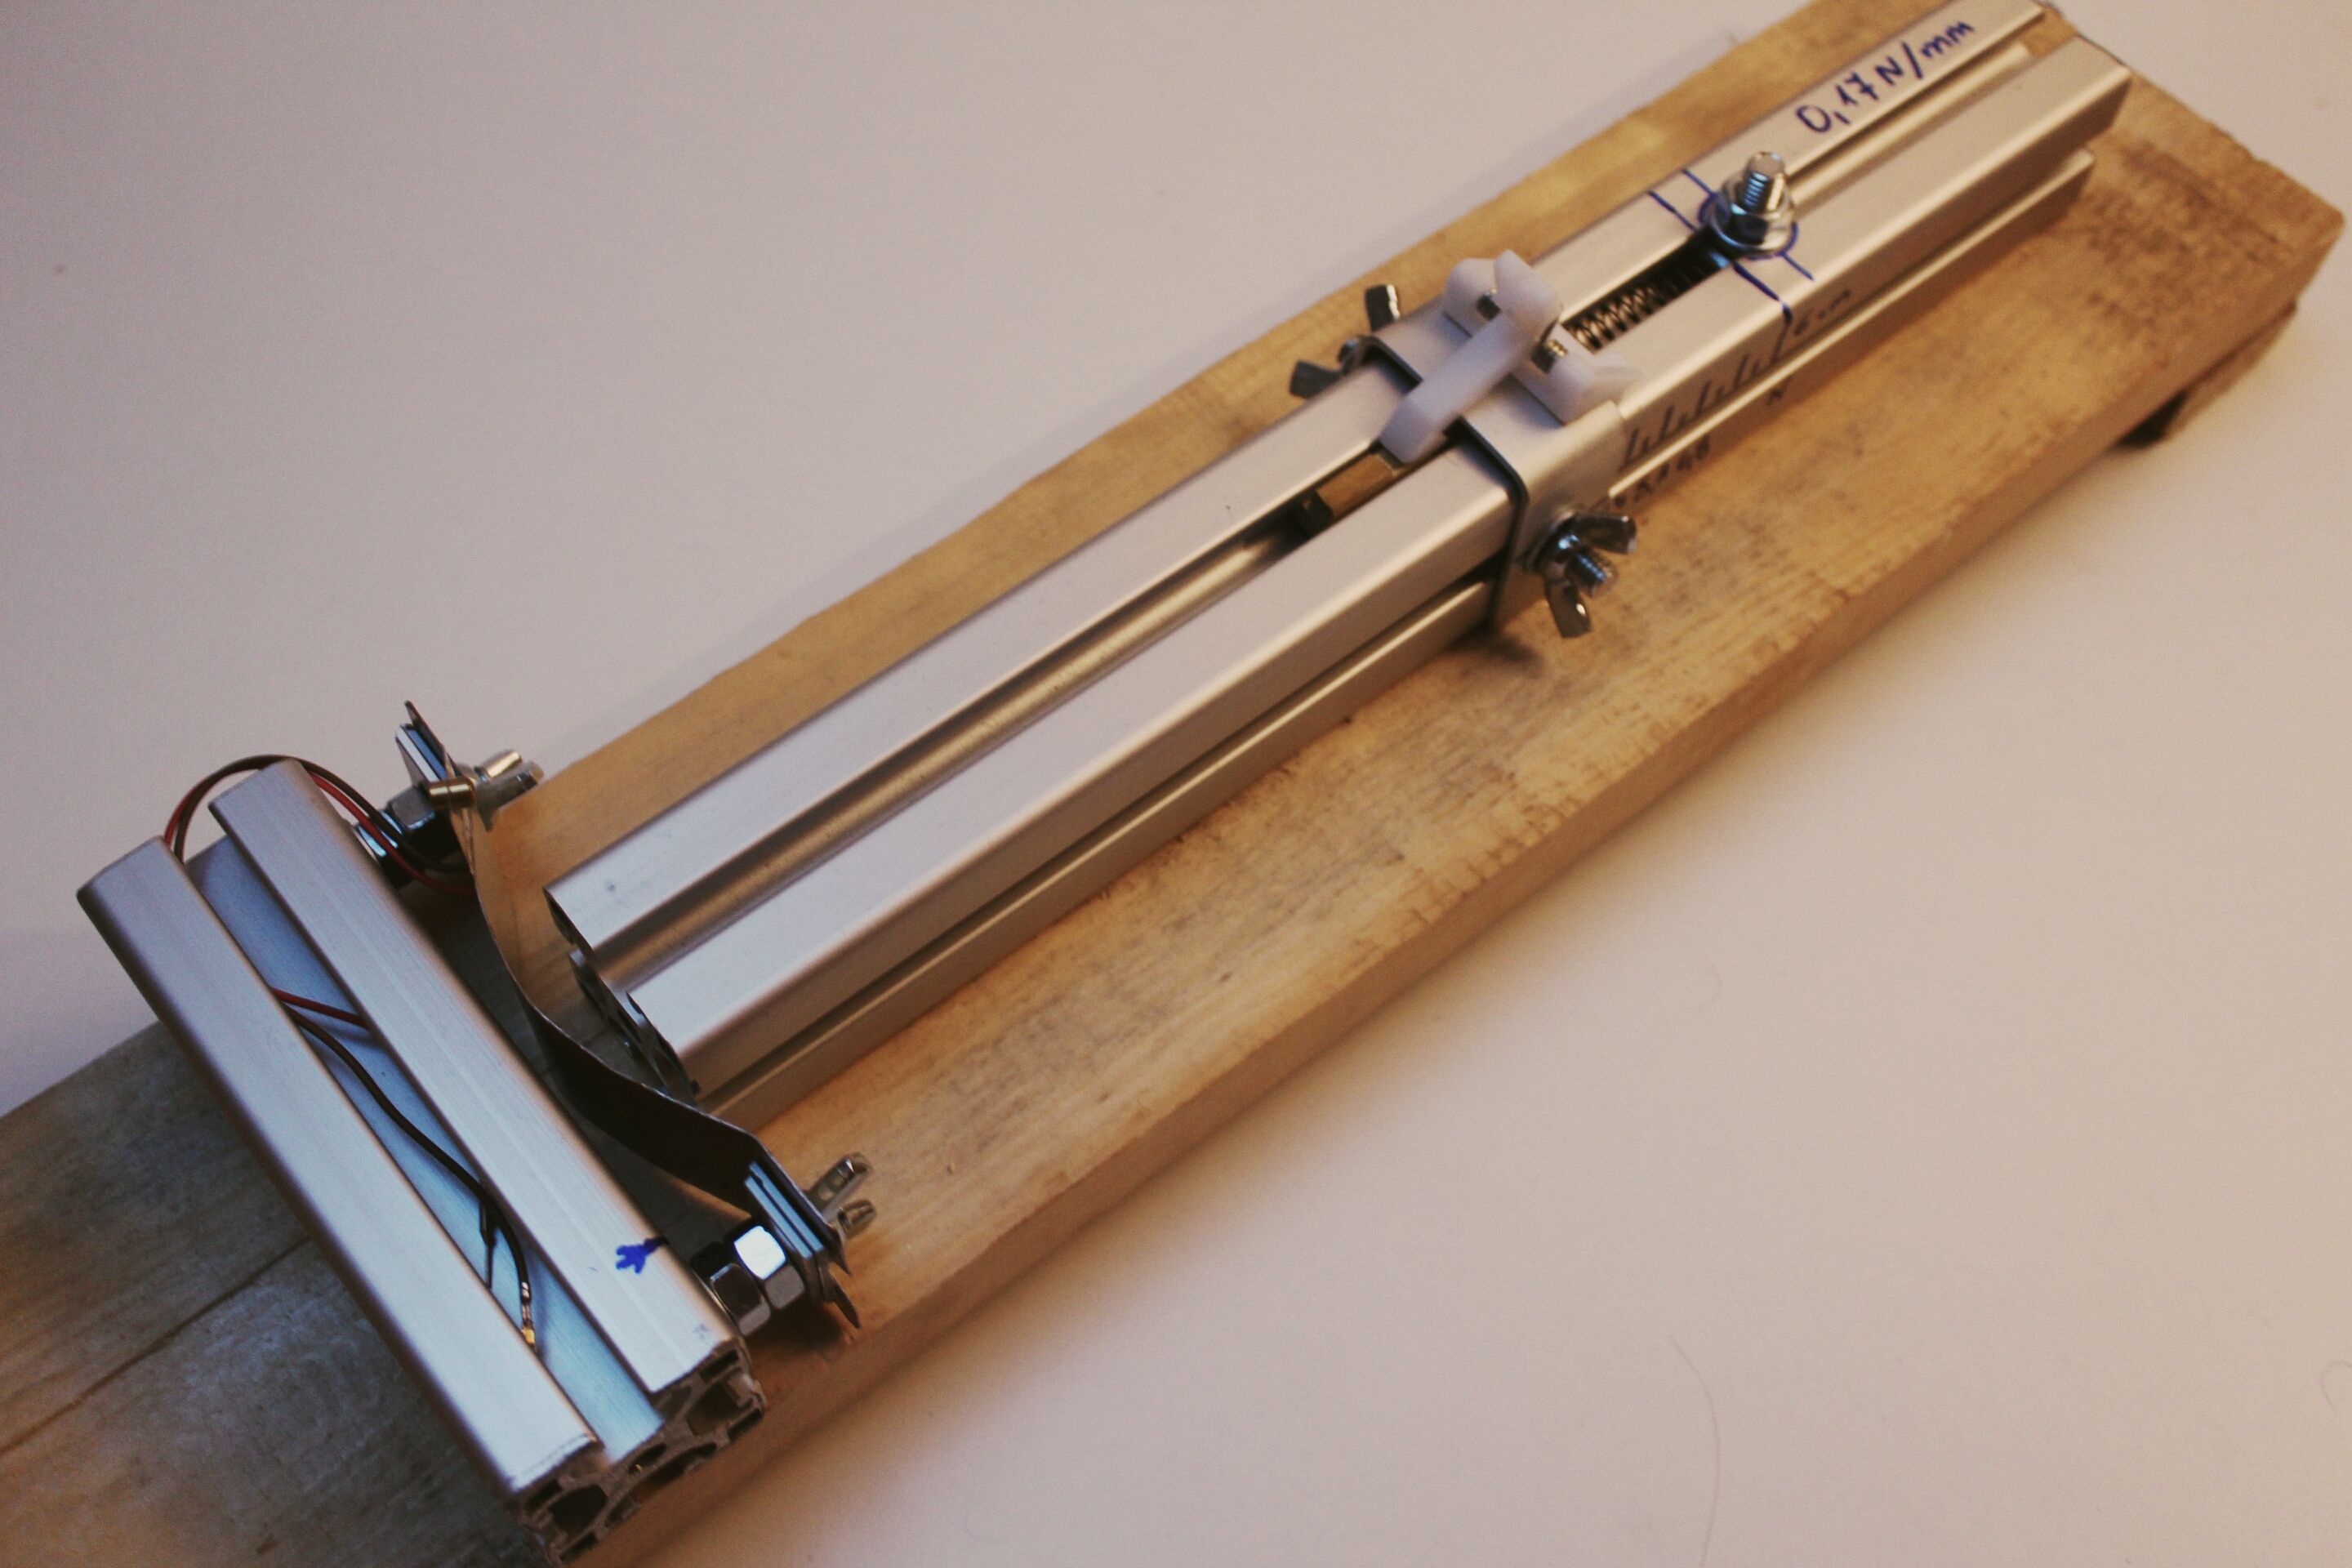
\includegraphics[width=\linewidth]{pictures/lab_stand.jpg}
%}
\caption{Realizacja stanowiska badawczego.}
\label{fig:test_stand_photo}
\end{figure}

Tak skonstruowane stanowisko pozwoliło uzyskać charakterystyki mechaniczne $E(x)$ i $p(x)$ przedstawione na Rys.\ref{fig:mech_char}. Gdyby wziąć pod uwagę możliwość wymiany sprężyny oraz elementu wprawianego w ruch otrzymanoby całą rodzinę charakterystyk, a przez to większą uniwersalność urządzenia.

\pgfplotsset{width=\linewidth,compat=1.3}



\begin{figure}[htbp]
\centering
    \begin{tikzpicture}
%    \pgfplotsset{
%    scale only axis,
%    scaled x ticks=base 10:3,
%    xmin=0, xmax=0.06
%}
      \begin{axis}[
          width=\linewidth, % Scale the plot to \linewidth
          grid=major, % Display a grid
          grid style={dashed,gray!30}, % Set the style
          xlabel=${\delta}x$ , % Set the labels
          ylabel=$E_k$,
          x unit=\si{\milli\metre}, % Set the respective units
          y unit=\si{\milli\joule},
          legend style={at={(0.5,-0.2)},anchor=north}, % Put the legend below the plot
          %x tick label style={rotate=90,anchor=east} % Display labels sideways
        ]
        \addplot[smooth,mark=*,blue] table[x=x,y=E-W,col sep=comma] {pomiary.csv};
        \label{plot_two}
        \addlegendentry{plot 2}
        \end{axis}


        \begin{axis}[
          axis y line*=right,
          axis x line=none,
          width=\linewidth, 
          ylabel=$p$,
          y unit=\si{\k\g\m\per\square\s},
        ] 
        \addlegendimage{/pgfplots/refstyle=plot_one}\addlegendentry{plot 1}
        \addplot[smooth,mark=x,red] table[x=x,y=p,col sep=comma] {pomiary.csv};
        \addlegendentry{plot 3} 
%        \legend{Plot, Plot2}
      \end{axis}
    
%      \begin{axis}[
%          width=\linewidth, % Scale the plot to \linewidth
%          grid=major, % Display a grid
%          grid style={dashed,gray!30}, % Set the style
%          xlabel=${\delta}x$ , % Set the labels
%          ylabel=$E_k$,
%          x unit=\si{\milli\metre}, % Set the respective units
%          y unit=\si{\milli\joule},
%          legend style={at={(0.5,-0.2)},anchor=north}, % Put the legend below the plot
%          %x tick label style={rotate=90,anchor=east} % Display labels sideways
%        ]
%        \addplot table[x=x,y=E-W,col sep=comma] {pomiary.csv};
%        \end{axis}
%        \begin{axis}[
%          axis y line*=right,
%          axis x line=none,
%          width=\linewidth, 
%          ylabel=$p$,
%          %y unit=\si{\k\g\m\per\square\s},
%        ] 
%        \addplot table[x=x,y=p,col sep=comma] {pomiary.csv}; 
%%        \legend{Plot, Plot2}
%      \end{axis}
    \end{tikzpicture}
\caption{Charakterystyka mechaniczna stanowiska badawczego.}
\label{fig:mech_char}
\end{figure}

